L'approvisionnement d'une multitude de métaux peut être étudié. Cinq métaux particulièrement critiques pour les technologies bas-carbone sont revus dans cette étude. Le contexte de chaque métal est donné dans les fiches suivantes.
Chaque fiche est introduite par un diagramme en barre horizontal. Ce diagramme utilise les dernières données disponibles pour exposer la répartition des réserves, de la production minière (extraction), de la production de métal raffiné (production) et éventuellement de la consommation.\\
\\
Sources des fiches métaux : \cite{brgm_fiche_2016},\cite{brgm_fiche_2016-1},\cite{brgm_fiche_2017},\cite{brgm_fiche_2018},\cite{brgm_fiche_2021},\cite{iea_role_2021}, \cite{usgs_rare_2021}

\begin{center}
    \boxput*(0,1){
        \colorbox{white}{Scénarios AIE}
    }{
    \setlength{\fboxsep}{15pt}
    \fbox{\begin{minipage}{14cm} 
    Plusieurs scénarios sont envisagés dans les publication de l'agence internationale de l'énergie.\\
    \\
    \textbf{STEPS} pour "Stated Policies Scenario". Le STEPS fournit une référence plus prudente pour l'avenir, car il ne tient pas pour acquis que les gouvernements atteindront tous les objectifs annoncés.\\
    \textbf{APS} pour "Announced Pledges Scenario". Un scénario qui suppose que tous les engagements climatiques pris par les gouvernements du monde entier, y compris les contributions déterminées au niveau national et les objectifs de zéro net à plus long terme, ainsi que les objectifs d'accès à l'électricité.\\
    \textbf{SDS} pour "Sustainable Development Scenario". SDS est un scénario normatif utilisé pour modéliser une trajectoire "bien en dessous de 2°C" ainsi que la réalisation d'autres objectifs de développement durable.\\
    \textbf{NZE} pour "Net Zero Emission by 2050". Un scénario qui définit une voie pour que le secteur mondial de l'énergie atteigne zéro émission nette de CO$_2$ d'ici 2050. Il ne s'appuie pas sur les réductions d'émissions extérieures au secteur de l'énergie pour atteindre ses objectifs. Il implique l'accès universel à l'électricité d'ici 2030.\\
    \\
    Source : \cite{iea_global_2022}
    
    \end{minipage}}
    }
\end{center}

\begin{figure}[!b]
    \centering
    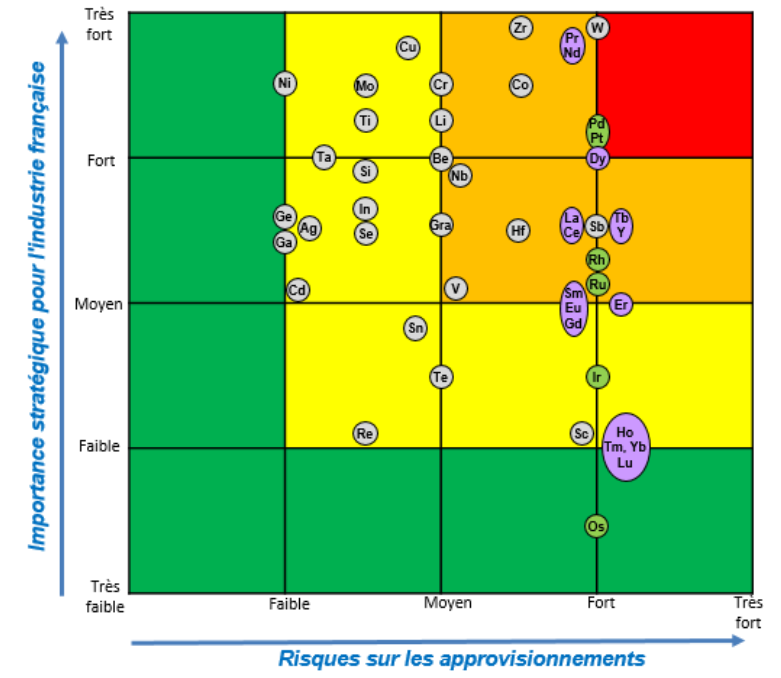
\includegraphics[width=0.6\textwidth]{Illustration métaux/martice.png}
    \caption{Criticite des métaux en France d'après \cite{brgm_marche_nodate}}
    \label{fig:my_label}
\end{figure}